% Template for Cogsci submission with R Markdown

% Stuff changed from original Markdown PLOS Template
\documentclass[10pt, letterpaper]{article}

\usepackage{cogsci}
\usepackage{pslatex}
\usepackage{float}
\usepackage{caption}

% amsmath package, useful for mathematical formulas
\usepackage{amsmath}

% amssymb package, useful for mathematical symbols
\usepackage{amssymb}

% hyperref package, useful for hyperlinks
\usepackage{hyperref}

% graphicx package, useful for including eps and pdf graphics
% include graphics with the command \includegraphics
\usepackage{graphicx}

% Sweave(-like)
\usepackage{fancyvrb}
\DefineVerbatimEnvironment{Sinput}{Verbatim}{fontshape=sl}
\DefineVerbatimEnvironment{Soutput}{Verbatim}{}
\DefineVerbatimEnvironment{Scode}{Verbatim}{fontshape=sl}
\newenvironment{Schunk}{}{}
\DefineVerbatimEnvironment{Code}{Verbatim}{}
\DefineVerbatimEnvironment{CodeInput}{Verbatim}{fontshape=sl}
\DefineVerbatimEnvironment{CodeOutput}{Verbatim}{}
\newenvironment{CodeChunk}{}{}

% cite package, to clean up citations in the main text. Do not remove.
\usepackage{apacite}

% KM added 1/4/18 to allow control of blind submission
\cogscifinalcopy

\usepackage{color}

% Use doublespacing - comment out for single spacing
%\usepackage{setspace}
%\doublespacing


% % Text layout
% \topmargin 0.0cm
% \oddsidemargin 0.5cm
% \evensidemargin 0.5cm
% \textwidth 16cm
% \textheight 21cm

\title{Understanding the impact of electronically-delivered parenting advice}


\author{{\large\bf Hanwen Vivian~Zhang} (\texttt{vivian3@stanford.edu}) \\ {\large\bf George~Kachergis} (\texttt{george.kachergis@gmail.com}) \\ {\large\bf Michael C.~Frank} (\texttt{mcfrank@stanford.edu}) \\  Department of Psychology, Stanford University \\  Palo Alto, CA 94301 USA}

\begin{document}

\maketitle

\begin{abstract}
Early parenting practices play an important role in shaping the future
outcomes of young children (Hart \& Risley, 1995; Heckman, 2006). In
particular, high quality early interactions and early language input
appear to facilitate more effective language learning and higher levels
of school performance. The rise in electronic parenting applications
(``apps'') holds the promise of delivering low-cost, positive
interventions on parenting style to a variety of different populations.
Of special interest are the parents of very young children, who are
often difficult to reach in other ways. Yet little is known about the
effects of communicating to parents through app-based interventions.
MTLD, types and tokens, joint attention, proportion of
nouns/verbs/adjectives, affect, concreteness, mean length of
utterance\ldots{}

\textbf{Keywords:}
digital parenting advice; joint attention; lexical diversity; guided
play;
\end{abstract}

\section{Introduction}\label{introduction}

Children spend a large portion of their waking time at play in their
environment. Playing with objects may allow them to discover hidden
features, as well as to build a causal understanding of how the objects
interact. Beyond learning object features, the laws of physics, and
causal relationships (e.g., Schulz \& Bonawitz, 2007), during play
children practice motor skills that help them effectively navigate their
world (Singer, Golinkoff, \& Hirsh-Pasek, 2006). Social play can help
children learn about human relationships, both through imitation of
adult behaviors and by experiencing and learning to process emotional
events (Singer et al., 2006).

\subsection{Guided Play Scaffolds
Learning}\label{guided-play-scaffolds-learning}

Children's early play behaviors are often assisted by more skilled and
knowledgeable play partners such as their caregivers and older siblings
(Kaye, 1970). Under such expert guidance, children are encouraged and
motivated to engage in more advanced play, undertaking explorations that
push the boundaries of what they would be able to do unaided (Vygotsky,
197X). These tutorial interactions have been shown to be a ``a crucial
feature of infancy and childhood'' (Wood, 1970). Thus, with the
knowledge of both play and tutorial interactions, guided play, ``where
children actively engage in pleasurable and seemingly spontaneous
activities under the direction of adults'' (Hirsh-Pasek, 2008), have
drawn researchers' interest. Weisberg showed that, with preschoolers,
guided play scaffolds the environment while still allowing children to
maintain a large degree of control, and it outperforms
direct-instruction approaches in encouraging a variety of positive
academic outcomes (Weisberg, Hirsh-Pasek and Golinkoff, 2013). Massey
specifically showed that guided play could facilitate children's
vocabulary and comprehensive language development and subsequent
literacy skills (Massey, 2013).

\subsection{Improving Parenting Practices and Language
Use}\label{improving-parenting-practices-and-language-use}

(early interventions on parenting practices can help children's
outcomes) Thus, including guided play in parenting practices early on is
important and should help with children's later performances. Suskind
did a parent-directed home-visiting intervention experiment in 2015, and
found that parents in experimental group have greater knowledge of
language development and this effect sustained after the experiment is
done. However, more interactive outcomes, like parent word type and
token numbers, child word types, conversational turn counts and child
vocalization counts, increased during the home-visiting but did not
sustain after four months of intervention (there are more detailed
sustainibility differences of these measure. should I make it more
clear?) (Susking et al., 2015). The fact that changes did not sustain
could be due to the intervention itself, or could merely be that
home-visiting is not sustainable enough for parents to easily and
constantly get parenting advice.

\subsection{Effectiveness of Digital
Delivery}\label{effectiveness-of-digital-delivery}

(apps are an easy way to deliver curated, age-appropriate parenting
advice --- but can we measure an influence on parent's language? and do
the interventions lead to children paying more attention?)

Digitally-delivered methods could address some logistic barriers to
face-to-face delivery methods. Bretenstein reviewed 11 studies on them
and showed good promise for the efficacy of interventions using
digitally-delivered methods. However, the parent and child outcomes
assessed in the review (e.g.infant positive behaviors, satisfaction,
emotional symptoms etc.) did not address the nature or quality of
parent-infant interactions at a detailed level, like if the
interventions lead to children paying more attention, or vocabulary
changes in parents' language usages. Thus, we want to conduct this
experiment to explore if and how digital scaffolding of activities
affect the social and linguistic characteristics of parent-child
ineractions.

The quality of parent-child interactions can be measured by both the
social engagement of parents (e.g., joint attention to objects in the
environment) and the quality of language (e.g., vocabulary diversity).
Although digitally-delivered activities are designed to promote learning
and cognitive development, it is unclear how they might affect these
dimensions of parent-child interactions. How does digital scaffolding of
activities affect the social and linguistic characteristics of parents'
speech to their children?

\section{Experiment 1}\label{experiment-1}

In Experiment 1, we invited parents of 6- to 24-month-old infants
visiting the Children's Discovery Museum in San Jose to complete
activities from the Kinedu app. Parents were randomly assigned to the
video group or the control group; parents in the video group watched a
video from the Kinedu app (matched to their child's age), and then
performed the activity with their child using the props from the video.
Parents in the control group did not watch a Kinedu video, instead they
were given the same props and were told to play with their infants as
they would at home. We found that compared to the control group, parents
who watched a Kinedu video spoke more words overall, but had lower
lexical diversity. They also made more bids for joint attention with
their infants, although these bids did not result in more episodes of
joint attention compared to the control group. In summary, following
digitally-scaffolded activities may cause parents to engage with and
speak more to children overall, but speak more repetitively.

\subsection{Method}\label{method}

\subsubsection{Participants.}\label{participants.}

60 infants aged 6-24 months and their parents participated in a museum
in northern California. We included infants who were exposed to English
at least 50 percent of the time or who were exposed less but whose
participating parent reported that they primarily speak English with
their child at home. {[}include specific demo info here?{]} - good to
include now, and we can comment it out if it's too much (the full
report/paper will have it)

\subsubsection{Materials.}\label{materials.}

Stimuli included videos from a commercial parenting application, Kinedu
Inc. The videos were designed to show activities parents could perform
with their child to foster cognitive and physical development, and were
targeted to the child's age and development. In each video, an adult and
child perform the activity while a narrator explains the activity and
its purpose. We selected two videos for each of three age groups in our
sample (6-11.9 months, 12-17.9 months, 18-23.94 months). More
information about the specific videos is available in the Appendix.
Participants were also given a set of props corresponding to those in
the video they watched, so that they could complete the activity. The
props associated with each video are listed in the Appendix.

Participants were randomly assigned to an Activity Video condition or
No-Video Control condition. Participants in the Activity Video condition
were assigned to one of the two videos available for their child's age
group. The No-Video Control condition was yoked to the Activity Video
condition such that for every participant in the Activity Video
condition who saw a particular video and received the associated props,
a participant in the No-Video Control condition received the same props
but did not watch the corresponding video. Parents also completed the
Parenting Attitudes Questionnaire (PAQ). The PAQ measures parents'
attitudes about parenting and child development along three dimensions:
rules and respect, early learning, and affection and attachment.

\subsection{Procedure.}\label{procedure.}

After providing informed consent, parents in the Activity Video
condition watched the assigned video on a laptop with headphones. To
ensure that parents could give the video their full attention, the
experimenter played with the infant with a set of toys (different from
the experimental props used in the study) while the video was being
played. Immediately following the video, each parent-child dyad was
provided with the props to complete the activity they had viewed. The
toys were placed on a large foam mat, and parents were instructed to sit
on the mat with their child and re-create the activity they had viewed
for a period of three minutes. In the No-Video control condition, after
consenting parents were told to play with their child as they would at
home with the provided props for a period of three minutes. They were
not given any additional instructions about how to use the props.

In both conditions, two video cameras were used to record the play
session from different angles, and parents were fitted with a wireless
audio recorder to record their speech to their child. After three
minutes of play had elapsed, parents were told they could stop playing
and cameras and audio were turned off. Parents were then asked to
complete the PAQ before being debriefed.

\subsubsection{Joint Attention Coding
Procedure.}\label{joint-attention-coding-procedure.}

Video of each session was coded for episodes of joint attention using
Datavyu software. The video taken at floor level was coded by default,
but the other video was referred to if the participants were not visible
or if there was a technological error with the first camera. For each
participant we coded for episodes of coordinated joint attention,
episodes of passive joint attention, and parental bids for joint
attention. We defined parental bids for joint attention as any attempt
to initiate joint attention (i.e label, point, or otherwise draw
attention to an object) that does not result in passive or coordinated
joint attention. If more than 3 seconds elapsed between bids, they were
coded as separate attempts. An episode of joint attention was considered
passive if both participants visually focused on an object for a minimum
of 3 seconds but the child did not acknowledge the parent. If either
participant looked away from the object for less than 3 seconds and then
returned to the same object it was considered part of the same period of
joint attention. Episodes joint attention were considered coordinated if
both participants visually focused on an object for a minimum of 3
seconds and at some point in the interaction the child indicated
awareness of interaction with some overt behavior toward the parent.
This could be looks to the parent's face, gestures, vocalizations, or
turn-taking. If either participant looked away for less than 3 seconds
and then returned to the same object, it was coded as part of the same
period of joint attention. A second coder independently coded a third of
the videos (i.e., 20 of the 60 videos, approximately equally distributed
across ages) to establish reliability. \% report reliability

\section{Results}\label{results}

The data was analyzed according to our preregistration:
\href{https://osf.io/2bpdf/}{link}.

\subsection{Lexical Diversity}\label{lexical-diversity}

We first calculated Type/Token Ratio (TTR) for each transcript. ..

Fig 1 - TTR, maybe also Total Tokens and Total Types (if subfigures fit)
(otherwise a table with mean and SD of tokens, types, and TTR) However,
note that TTR is a measure that is correlated with the length of a text.
\ldots{} MTLD is a better measure of lexical diversity (McCarthy \&
Jarvis, 2010).

\begin{CodeChunk}
\begin{figure}[H]

{\centering 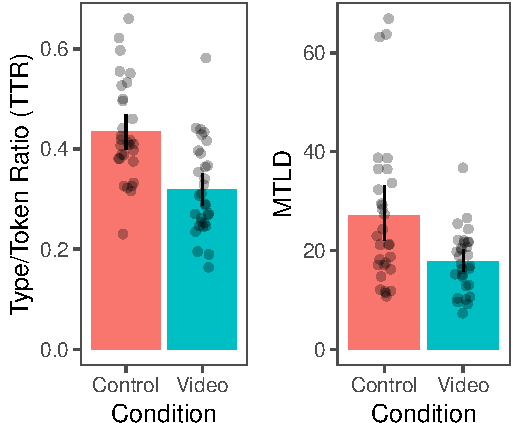
\includegraphics{figs/e1lex_div-1} 

}

\caption[Mean lexical diversity scores by condition (left]{Mean lexical diversity scores by condition (left: Type/Token ratio, right: MTLD) in Experiment 1.}\label{fig:e1lex_div}
\end{figure}
\end{CodeChunk}

Word tokens and word types

\begin{CodeChunk}
\begin{figure}[H]

{\centering 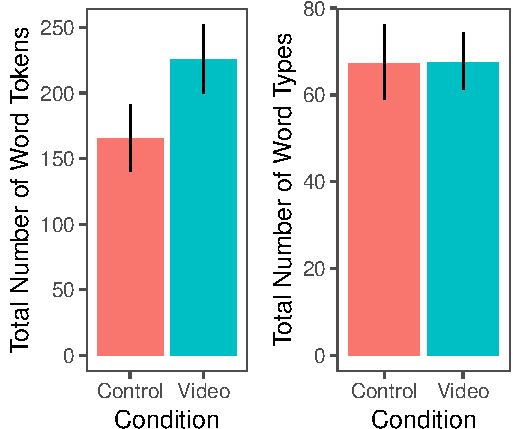
\includegraphics{figs/e1token_type-1} 

}

\caption[Mean number of word types and word tokens by condition in Experiment 1]{Mean number of word types and word tokens by condition in Experiment 1.}\label{fig:e1token_type}
\end{figure}
\end{CodeChunk}

\subsection{Joint Attention}\label{joint-attention}

\section{Experiment 2}\label{experiment-2}

In Experiment 2 we attempt to replicate the findings from Experiment 1
with a restricted number of preregistered predictions. We will
additionally include a second control condition, in which the same
activities are described in written form, rather than being demonstrated
in video. This manipulation will help determine what the contribution of
the video demonstration is in producing the observed effects on
parent-child interactions.

\subsection{Method}\label{method-1}

\subsubsection{Participants.}\label{participants.-1}

84 infants aged 12-24 months and their parents participated in the same
museum as Experiment 1. We included infants who were exposed to English
at least 75 percent of the time or who were exposed less but whose
participating parent reported that they primarily speak English with
their child at home. {[}specific demo info{]}

\subsubsection{Materials.}\label{materials.-1}

The design of Experiment 2 was similar to that of Experiment 1, except
that instead of a No-Video control condition, parents instead watched a
video that was generally related to child development research, but did
not give any specific instructions about how to interact with infants or
children. This was to control for the possibility that differences in
language output and joint attention in Experiment 1 could be due to
simply cuing parents to think about infants' learning and cognitive
development. The videos presented in the Control Video condition were
media clips (available on YouTube) of developmental psychologists
explaining their research interleaved with footage of infants or
toddlers engaged in developmental research studies. Thus, the content of
the videos superficially matched those in the Activity Video condition,
but did not suggest any particular activities. The videos were trimmed
to approximately match the average video length in the Activity Video
condition (2 minutes ??).

\subsubsection{Procedure.}\label{procedure.-1}

The procedure for Experiment 2 matched that of Experiment 1, except that
parents in the Control Video condition watched a control video before
the play session. Consistent with the No-Video control condition in
Experiment 1, parents in the Control Video condition were told to play
with their child as they would at home, and were not given additional
instructions.

\section{Results}\label{results-1}

\begin{CodeChunk}
\begin{figure}[H]

{\centering 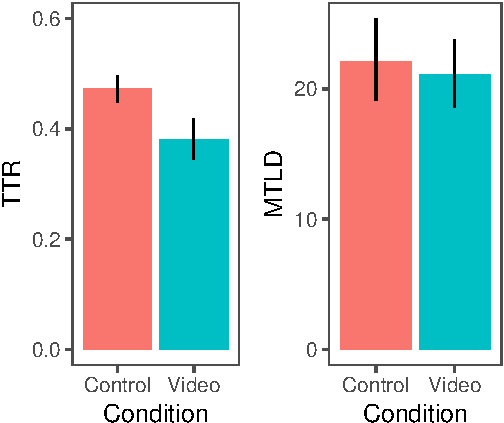
\includegraphics{figs/e2TTR-1} 

}

\caption[How to do subfigures?]{How to do subfigures?}\label{fig:e2TTR}
\end{figure}
\end{CodeChunk}

\begin{CodeChunk}
\begin{figure}[H]

{\centering 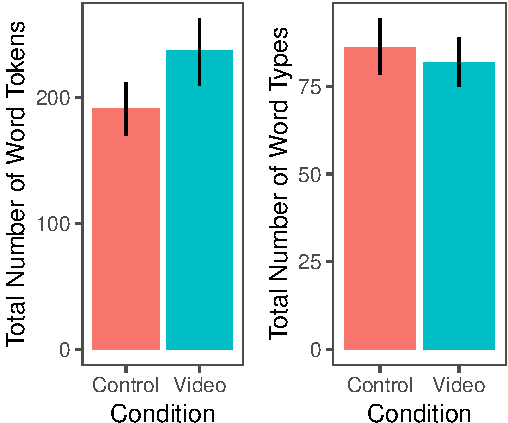
\includegraphics{figs/e2MTLD-1} 

}

\caption[One column image]{One column image.}\label{fig:e2MTLD}
\end{figure}
\end{CodeChunk}

\subsection{Lexical Diversity}\label{lexical-diversity-1}

\subsection{Joint Attention}\label{joint-attention-1}

\section{Discussion}\label{discussion}

\subsection{Footnotes}\label{footnotes}

Indicate footnotes with a number\footnote{Sample of the first
footnote.} in the text. You can also use markdown formatting to include
footnotes using this syntax.\footnote{Sample of a markdown footnote.}

\subsection{Two-column images}\label{two-column-images}

You might want to display a wide figure across both columns. To do this,
you change the \texttt{fig.env} chunk option to \texttt{figure*}. To
align the image in the center of the page, set \texttt{fig.align} option
to \texttt{center}. To format the width of your caption text, you set
the \texttt{num.cols.cap} option to \texttt{2}.

\subsection{Tables}\label{tables}

Number tables consecutively; place the table number and title (in 10
point) above the table with one line space above the caption and one
line space below it, as in Table 1. You may float tables to the top or
bottom of a column, set wide tables across both columns.

You can use the xtable function in the xtable package.

\section{References}\label{references}

\setlength{\parindent}{-0.1in} \setlength{\leftskip}{0.125in} \noindent

\hypertarget{refs}{}
\hypertarget{ref-Hart1995}{}
Hart, B., \& Risley, T. R. (1995). \emph{Meaningful differences in the
everyday experience of young american children}. Baltimore, MD: Brookes.

\hypertarget{ref-Heckman2006}{}
Heckman, J. J. (2006). Skill formation and the economics of investing in
disadvantaged children. \emph{Science}, \emph{312}(5782), 1900--1902.
\url{http://doi.org/10.1126/science.1128898}

\hypertarget{ref-McCarthy2010}{}
McCarthy, P. M., \& Jarvis, S. (2010). MTLD, vocd-d, and hd-d: A
validation study of sophisticated approaches to lexical diversity
assessment. \emph{Behavior Research Methods}, \emph{42}(2), 381--392.

\hypertarget{ref-Schulz2007}{}
Schulz, L., \& Bonawitz, E. (2007). Serious fun: Preschoolers engage in
more exploratory play when evidence is confounded. \emph{Developmental
Psychology}, \emph{43}(4), 1045--1050.

\hypertarget{ref-Singer2006}{}
Singer, D. G., Golinkoff, R. M., \& Hirsh-Pasek, K. (Eds.). (2006).
\emph{Play = learning: How play motivates and enhances children's
cognitive and social-emotional growth}. New York, NY: Oxford University
Press.

\hypertarget{ref-Suskind2015}{}
Susking, D. L., Leffel, K. R., Graf, E., Hernandez, M. W., Gunderson, E.
A., Sapolich, S. G., \ldots{} Levine, S. C. (2015). A parent-directed
language intervention for children of low socioeconomic status: A
randomized controlled pilot study. \emph{Journal of Child Language}.
\url{http://doi.org/10.1017/S0305000915000033}

\bibliographystyle{apacite}


\end{document}
